\section{Results}
\label{sec:results}

\subsection{Random versus chronological split}

\begin{table}[t]
\caption{Random versus chronological split. Mean $\pm$ standard deviation over 5 seeds; $\Delta$ = chronological $-$ random.}
\label{tab:main}
\small
\begin{tabular}{llrrrrrr}
\toprule
 &  & \multicolumn{3}{c}{PR-AUC} & \multicolumn{3}{c}{ROC-AUC} \\
\cmidrule(lr){3-5}\cmidrule(lr){6-8}
Dataset & Model & Random & Chrono. & $\Delta$ & Random & Chrono. & $\Delta$ \\
\midrule
IEEE-CIS & Logistic regression & 0.474 {\scriptsize$\pm$ 0.006} & 0.360 {\scriptsize$\pm$ 0.001} & $-$0.114 & 0.865 {\scriptsize$\pm$ 0.005} & 0.840 {\scriptsize$\pm$ 0.001} & $-$0.025 \\
 & Random forest & 0.727 {\scriptsize$\pm$ 0.006} & 0.523 {\scriptsize$\pm$ 0.004} & $-$0.204 & 0.942 {\scriptsize$\pm$ 0.003} & 0.900 {\scriptsize$\pm$ 0.001} & $-$0.042 \\
 & XGBoost & 0.864 {\scriptsize$\pm$ 0.006} & 0.594 {\scriptsize$\pm$ 0.003} & $-$0.270 & 0.972 {\scriptsize$\pm$ 0.002} & 0.916 {\scriptsize$\pm$ 0.004} & $-$0.056 \\
 & LightGBM & 0.866 {\scriptsize$\pm$ 0.006} & 0.596 {\scriptsize$\pm$ 0.003} & $-$0.270 & 0.973 {\scriptsize$\pm$ 0.002} & 0.922 {\scriptsize$\pm$ 0.002} & $-$0.052 \\
 & MLP & 0.713 {\scriptsize$\pm$ 0.009} & 0.452 {\scriptsize$\pm$ 0.014} & $-$0.261 & 0.932 {\scriptsize$\pm$ 0.004} & 0.857 {\scriptsize$\pm$ 0.007} & $-$0.075 \\
\addlinespace
ULB & Logistic regression & 0.762 {\scriptsize$\pm$ 0.042} & 0.787 {\scriptsize$\pm$ 0.000} & $+$0.024 & 0.983 {\scriptsize$\pm$ 0.007} & 0.986 {\scriptsize$\pm$ 0.000} & $+$0.003 \\
 & Random forest & 0.851 {\scriptsize$\pm$ 0.023} & 0.797 {\scriptsize$\pm$ 0.010} & $-$0.055 & 0.980 {\scriptsize$\pm$ 0.004} & 0.980 {\scriptsize$\pm$ 0.010} & $+$0.000 \\
 & XGBoost & 0.856 {\scriptsize$\pm$ 0.036} & 0.796 {\scriptsize$\pm$ 0.013} & $-$0.059 & 0.986 {\scriptsize$\pm$ 0.006} & 0.984 {\scriptsize$\pm$ 0.004} & $-$0.002 \\
 & LightGBM & 0.859 {\scriptsize$\pm$ 0.027} & 0.781 {\scriptsize$\pm$ 0.018} & $-$0.078 & 0.983 {\scriptsize$\pm$ 0.006} & 0.974 {\scriptsize$\pm$ 0.025} & $-$0.009 \\
 & MLP & 0.845 {\scriptsize$\pm$ 0.016} & 0.811 {\scriptsize$\pm$ 0.013} & $-$0.034 & 0.977 {\scriptsize$\pm$ 0.006} & 0.986 {\scriptsize$\pm$ 0.004} & $+$0.009 \\
\bottomrule
\end{tabular}
\end{table}


\paragraph{IEEE-CIS}
Table~\ref{tab:main} gives the main comparison. Every model scores considerably lower when it is evaluated on later transactions. \prauc{} is lower by between \num{ieee.min.drop.pr} for logistic regression and \num{ieee.max.drop.pr} for the boosted models, which corresponds to \num{ieee.min.rel.pr}\% to \num{ieee.max.rel.pr}\% of the random-split score, and the mean difference over the five models is \num{ieee.mean.drop.pr}. These differences are far larger than the variation between seeds, and the bootstrap 95\% interval of the smallest one, for logistic regression, is [\num{ieee.lr.ci.lo}, \num{ieee.lr.ci.hi}].

\rocauc{} reflects the same effect but understates it. LightGBM moves from \num{ieee.lgbm.random.roc} to \num{ieee.lgbm.chrono.roc} on \rocauc{}, a change that would be easy to overlook in a results table, while its \prauc{} falls by about a third.

\paragraph{ULB}
On ULB, the three tree-based models lose \num{ulb.rf.drop.pr} to \num{ulb.lgbm.drop.pr} \prauc{} and their bootstrap intervals exclude zero. The MLP loses \num{ulb.mlp.drop.pr} with an interval of [\num{ulb.mlp.ci.lo}, \num{ulb.mlp.ci.hi}], and logistic regression shows no loss. Two caveats apply even to the tree-model result. The dataset is small, with \num{ulb.testfraud} fraud cases in the chronological test set, and the random-split score itself has a standard deviation of \num{ulb.rf.random.pr.sd} to \num{ulb.lr.random.pr.sd} across seeds, which is comparable to the differences between models that studies on this dataset report. In addition, as the next subsection shows, most of this drop is not attributable to leakage.

\paragraph{Model rankings}
On IEEE-CIS, the split does not change the order of the models (Kendall's $\tau=\num{ieee.tau.pr}$ between the two \prauc{} rankings), but it changes the distances between them. The spread between the best and the worst model shrinks from \num{ieee.range.random.pr} to \num{ieee.range.chrono.pr}. On ULB, the random split ranks the tree ensembles well ahead of logistic regression, whereas under the chronological split all five models fall within \num{ulb.range.chrono.pr} of each other and the order changes ($\tau=\num{ulb.tau.pr}$). Given the noise on ULB, we interpret this as the absence of a detectable difference between models rather than as a new ranking.

\subsection{Is the later period simply harder?}
\label{sec:controls}

A lower score on the last 20\% of the timeline could indicate that those weeks are harder, rather than that the random split leaked information. Table~\ref{tab:controls} reports the two controls that score both protocols on the same transactions.

\begin{table}[t]
\caption{Controls that score both protocols on the same transactions (\prauc{}). Left: random-split models scored only on their test transactions inside the chronological test period, against the chronological models. Right: five-fold cross-validation with random folds against contiguous time blocks.}
\label{tab:controls}
\small
\begin{tabular}{llrrrrrr}
\toprule
 & & \multicolumn{3}{c}{Same test period} & \multicolumn{3}{c}{Five-fold cross-validation} \\
\cmidrule(lr){3-5}\cmidrule(lr){6-8}
Dataset & Model & Random & Chrono. & $\Delta$ & Random folds & Time blocks & $\Delta$ \\
\midrule
IEEE-CIS & Logistic regression & 0.432 & 0.360 & $-$0.072 & 0.469 & 0.410 & $-$0.059 \\
 & Random forest & 0.725 & 0.523 & $-$0.202 & -- & -- & -- \\
 & XGBoost & 0.871 & 0.594 & $-$0.277 & -- & -- & -- \\
 & LightGBM & 0.870 & 0.598 & $-$0.273 & -- & -- & -- \\
 & MLP & 0.714 & 0.452 & $-$0.262 & 0.710 & 0.495 & $-$0.214 \\
\addlinespace
ULB & Logistic regression & 0.762 & 0.787 & $+$0.024 & 0.752 & 0.775 & $+$0.023 \\
 & Random forest & 0.771 & 0.797 & $+$0.026 & 0.850 & 0.790 & $-$0.060 \\
 & XGBoost & 0.765 & 0.796 & $+$0.031 & 0.853 & 0.792 & $-$0.061 \\
 & LightGBM & 0.753 & 0.781 & $+$0.028 & 0.846 & 0.787 & $-$0.059 \\
 & MLP & 0.775 & 0.811 & $+$0.036 & -- & -- & -- \\
\bottomrule
\end{tabular}
\end{table}


\paragraph{IEEE-CIS}
Restricting the random-split models to the test transactions that fall inside the chronological test period, about \num{ieee.matched.nfraud} fraud cases per seed, leaves their scores essentially unchanged for four of the five models. The random forest scores \num{ieee.rf.matched.pr} on that period compared with \num{ieee.rf.random.pr} overall, and LightGBM scores \num{ieee.lgbm.matched.pr} compared with \num{ieee.lgbm.random.pr}. The period is therefore not harder for these models, and what they lose under the chronological split is consistent with the benefit of having trained on transactions from the same weeks. Logistic regression is the exception. It scores \num{ieee.lr.matched.pr} on that period, so about a third of its drop reflects a harder period and two thirds the split. The cross-validation control agrees with this picture. With every transaction tested exactly once under both schemes, contiguous time blocks give lower \prauc{} than random folds for every model, and when averaged over the models the difference is positive in each of the five blocks (\num{ieee.blocks.mindrop} to \num{ieee.blocks.maxdrop}).

\paragraph{ULB}
On ULB, the controls lead to a different conclusion. Scored only on the final period, the random-split models do no better than the chronological ones, and in fact score slightly lower for all five models, although with about \num{ulb.matched.nfraud} fraud cases per seed the estimate is noisy. The drop in Table~\ref{tab:main} is therefore largely attributable to a harder final period. Cross-validation shows that interleaving does help the non-linear models on ULB, by 0.06 to 0.07 on average, but the benefit is uneven across the two days. Averaged over the models, it is \num{ulb.block1.drop} in the first of the five time blocks, \num{ulb.block3.drop} and \num{ulb.block4.drop} in the third and fourth, and absent in the second (\num{ulb.block2.drop}) and in the fifth (\num{ulb.block5.drop}), the fifth being the block that a chronological split tests. The controls are therefore necessary for interpreting the ULB result, and two days of data with \num{ulb.fraud} fraud cases do not support stronger conclusions.

\subsection{Different periods, label delay and time since training}

\begin{figure}[htbp]
\centering
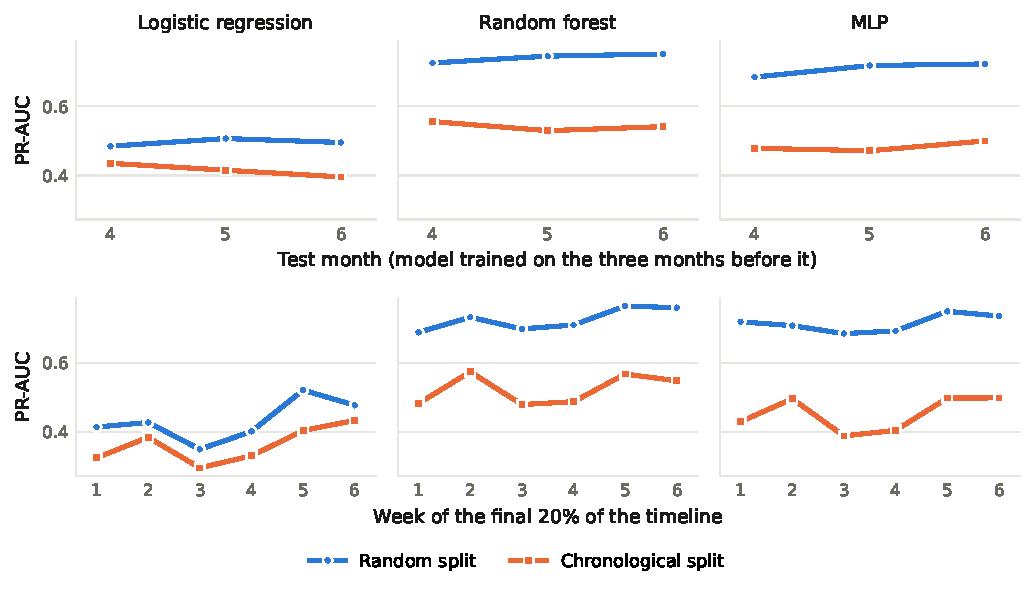
\includegraphics[width=\linewidth]{generated/fig_time.pdf}
\caption{IEEE-CIS. Top: \prauc{} on each rolling window, for a model trained on the three preceding months and for a random split of the same four months. Bottom: \prauc{} of the main-comparison models on each week of the final 20\% of the timeline, where random-split models are scored on their test transactions from that week.}
\Description{Two rows of five small line charts, one column per model. In every panel the random-split line lies above the chronological line. In the top row both lines are roughly flat across test months four to six. In the bottom row both lines move together across six weeks and the distance between them stays about the same.}
\label{fig:time}
\end{figure}

The top row of Figure~\ref{fig:time} repeats the comparison on three different four-month windows of IEEE-CIS. The random split scores higher than the chronological one for every model in every window, with differences ranging from \num{ieee.roll.mindrop} to \num{ieee.roll.maxdrop} and averaging \num{ieee.roll.meandrop}.

Removing the last seven days before the test period from the training data, to mimic label delay, has a small additional cost. Depending on the model, \prauc{} falls by a further \num{ieee.min.gap7.drop} to \num{ieee.max.gap7.drop}.

The bottom row of Figure~\ref{fig:time} follows the models through the six weeks of the test period. If the gap were caused by gradual drift, the chronological models would start close to the random-split ones and fall away over time. Instead, the gap is already close to its full size in the first week after the training cut-off, and over the six weeks it fluctuates and widens only slightly for the boosted models. The two curves rise and fall together, which reflects weeks that are easier or harder for any model. The advantage conferred by the random split is therefore lost as soon as training and test transactions are no longer interleaved (Section~\ref{sec:mechanism}).

\subsection{Alert budgets}

\begin{table}[t]
\caption{Alert-budget metrics under the two splits: share of fraud cases (recall) and of fraud value caught when the highest-scored 0.5\% or 1\% of test transactions are flagged.}
\label{tab:budget}
\small
\begin{tabular}{llrrrrrrrrr}
\toprule
 &  & \multicolumn{3}{c}{Recall at 0.5\% budget} & \multicolumn{3}{c}{Recall at 1\% budget} & \multicolumn{3}{c}{Value recall at 1\% budget} \\
\cmidrule(lr){3-5}\cmidrule(lr){6-8}\cmidrule(lr){9-11}
Dataset & Model & Random & Chrono. & $\Delta$ & Random & Chrono. & $\Delta$ & Random & Chrono. & $\Delta$ \\
\midrule
IEEE-CIS & Logistic regression & 0.138 {\scriptsize$\pm$ 0.001} & 0.110 {\scriptsize$\pm$ 0.001} & -0.027 & 0.249 {\scriptsize$\pm$ 0.003} & 0.197 {\scriptsize$\pm$ 0.001} & -0.052 & 0.164 {\scriptsize$\pm$ 0.007} & 0.133 {\scriptsize$\pm$ 0.001} & -0.031 \\
 & Random forest & -- & -- & -- & -- & -- & -- & -- & -- & -- \\
 & XGBoost & -- & -- & -- & -- & -- & -- & -- & -- & -- \\
 & LightGBM & -- & -- & -- & -- & -- & -- & -- & -- & -- \\
 & MLP & 0.143 {\scriptsize$\pm$ 0.000} & 0.133 {\scriptsize$\pm$ 0.001} & -0.010 & 0.283 {\scriptsize$\pm$ 0.000} & 0.235 {\scriptsize$\pm$ 0.003} & -0.049 & 0.214 {\scriptsize$\pm$ 0.009} & 0.163 {\scriptsize$\pm$ 0.002} & -0.051 \\
\addlinespace
ULB & Logistic regression & 0.878 {\scriptsize$\pm$ 0.028} & 0.867 {\scriptsize$\pm$ 0.000} & -0.011 & 0.890 {\scriptsize$\pm$ 0.026} & 0.875 {\scriptsize$\pm$ 0.007} & -0.015 & 0.763 {\scriptsize$\pm$ 0.065} & 0.695 {\scriptsize$\pm$ 0.001} & -0.068 \\
 & Random forest & 0.878 {\scriptsize$\pm$ 0.029} & 0.832 {\scriptsize$\pm$ 0.031} & -0.046 & 0.890 {\scriptsize$\pm$ 0.028} & 0.856 {\scriptsize$\pm$ 0.026} & -0.034 & 0.773 {\scriptsize$\pm$ 0.083} & 0.737 {\scriptsize$\pm$ 0.053} & -0.036 \\
 & XGBoost & 0.882 {\scriptsize$\pm$ 0.025} & 0.819 {\scriptsize$\pm$ 0.007} & -0.063 & 0.906 {\scriptsize$\pm$ 0.023} & 0.853 {\scriptsize$\pm$ 0.019} & -0.053 & 0.821 {\scriptsize$\pm$ 0.108} & 0.779 {\scriptsize$\pm$ 0.027} & -0.043 \\
 & LightGBM & 0.880 {\scriptsize$\pm$ 0.023} & 0.824 {\scriptsize$\pm$ 0.030} & -0.056 & 0.892 {\scriptsize$\pm$ 0.015} & 0.853 {\scriptsize$\pm$ 0.025} & -0.039 & 0.767 {\scriptsize$\pm$ 0.056} & 0.794 {\scriptsize$\pm$ 0.061} & +0.027 \\
 & MLP & 0.882 {\scriptsize$\pm$ 0.019} & 0.861 {\scriptsize$\pm$ 0.015} & -0.020 & 0.898 {\scriptsize$\pm$ 0.020} & 0.883 {\scriptsize$\pm$ 0.011} & -0.015 & 0.788 {\scriptsize$\pm$ 0.044} & 0.835 {\scriptsize$\pm$ 0.081} & +0.047 \\
\bottomrule
\end{tabular}
\end{table}


Table~\ref{tab:budget} translates the comparison into review workload. On IEEE-CIS, fraud accounts for \num{ieee.rate}\% of transactions, so a 0.5\% or 1\% budget is smaller than the fraud volume and recall is capped. Within that cap, the top of the ranking holds up comparatively well. At a 1\% budget, the precision of LightGBM's alerts is \num{ieee.lgbm.random.p01} under the random split and \num{ieee.lgbm.chrono.p01} under the chronological one, although for logistic regression and the MLP it falls to \num{ieee.lr.chrono.p01} and \num{ieee.mlp.chrono.p01}. The inflation is concentrated deeper in the ranking. At a 5\% budget, which is large enough to contain every fraud case, LightGBM catches \num{ieee.lgbm.random.r05} of fraud cases and \num{ieee.lgbm.random.v05} of fraud value under the random split, but \num{ieee.lgbm.chrono.r05} and \num{ieee.lgbm.chrono.v05} on future transactions.

On IEEE-CIS, value recall is lower than recall for every model at the 1\% budget, because the fraud cases that are easiest to rank at the top are smaller than average, so counting cases overstates the value protected. On ULB, the alert-budget metrics change little, consistent with Section~\ref{sec:controls}.

\subsection{Oversampling before the split}

\begin{table}[t]
\caption{Oversampling leak under a random split. ``As reported'' scores the flawed pipeline on its own oversampled test set; ``genuine test rows'' scores the same models on the genuine transactions of that test set. Mean over 5 seeds.}
\label{tab:smote}
\small
\begin{tabular}{llrrrrrrrr}
\toprule
 &  & \multicolumn{2}{c}{\shortstack{Class\\weights}} & \multicolumn{2}{c}{\shortstack{SMOTE on\\training rows}} & \multicolumn{2}{c}{\shortstack{SMOTE before split,\\as reported}} & \multicolumn{2}{c}{\shortstack{SMOTE before split,\\genuine test rows}} \\
\cmidrule(lr){3-4}\cmidrule(lr){5-6}\cmidrule(lr){7-8}\cmidrule(lr){9-10}
Dataset & Model & PR-AUC & F1 & PR-AUC & F1 & PR-AUC & F1 & PR-AUC & F1 \\
\midrule
IEEE-CIS & Logistic regression & 0.476 & 0.442 & 0.449 & 0.234 & 0.891 & 0.789 & 0.456 & 0.241 \\
 & Random forest & 0.677 & 0.629 & 0.598 & 0.578 & 0.998 & 0.985 & 0.751 & 0.698 \\
 & XGBoost & -- & -- & -- & -- & -- & -- & -- & -- \\
 & LightGBM & -- & -- & -- & -- & -- & -- & -- & -- \\
 & MLP & 0.606 & 0.589 & 0.563 & 0.448 & 0.998 & 0.986 & 0.926 & 0.797 \\
\addlinespace
ULB & Logistic regression & 0.762 & 0.776 & 0.761 & 0.110 & 0.990 & 0.943 & 0.742 & 0.112 \\
 & Random forest & 0.851 & 0.851 & 0.856 & 0.718 & 1.000 & 1.000 & 0.986 & 0.855 \\
 & XGBoost & 0.856 & 0.854 & 0.867 & 0.787 & 1.000 & 1.000 & 0.994 & 0.898 \\
 & LightGBM & 0.859 & 0.856 & 0.854 & 0.729 & 1.000 & 1.000 & 0.890 & 0.846 \\
 & MLP & 0.845 & 0.768 & 0.835 & 0.790 & 1.000 & 1.000 & 0.991 & 0.876 \\
\bottomrule
\end{tabular}
\end{table}


Table~\ref{tab:smote} shows the second leak. Applied to the whole dataset before a random split, SMOTE produces the near-perfect figures familiar from the literature. On its own oversampled test set, the flawed pipeline reports a \prauc{} of \num{ulb.min.leakrep.pr} or more for every model on ULB and between \num{ieee.min.leakrep.pr} and \num{ieee.max.leakrep.pr} on IEEE-CIS, with correspondingly high F1 scores.

Part of this is an artifact of the test set, which is half synthetic fraud and no longer has the real class ratio. Scoring the same fitted models on only the genuine test transactions indicates, however, that real information has leaked as well. On ULB, XGBoost reaches \num{ulb.xgb.leakreal.pr}, the random forest \num{ulb.rf.leakreal.pr} and the MLP \num{ulb.mlp.leakreal.pr} on genuine transactions, compared with \num{ulb.xgb.smote.pr}, \num{ulb.rf.smote.pr} and \num{ulb.mlp.smote.pr} when only the training rows are oversampled. On IEEE-CIS, the MLP goes from \num{ieee.mlp.smote.pr} to \num{ieee.mlp.leakreal.pr} and the random forest from \num{ieee.rf.smote.pr} to \num{ieee.rf.leakreal.pr}, while the boosted models gain less (\num{ieee.lgbm.smote.pr} to \num{ieee.lgbm.leakreal.pr} for LightGBM). The mechanism is that a synthetic training point is placed on the segment between a fraud case and one of its neighbors, so that when the fraud case is assigned to the test set, the training set contains points immediately next to it that are labeled as fraud.

Logistic regression shows no measurable benefit from the leak on either dataset (\num{ulb.lr.leakreal.pr} compared with \num{ulb.lr.smote.pr} on ULB), which is what one would expect of a linear boundary that cannot exploit a small number of local points. The leak thus behaves like a memorization effect. It is not detectable for the linear model and is present, in varying size, for every non-linear one. LightGBM on ULB reaches 0.98 or more in four of five seeds, and in the fifth its training diverged, which reduces the mean to \num{ulb.lgbm.leakreal.pr}.

A secondary result is that SMOTE applied correctly does not improve on tuned class weights. On IEEE-CIS it is worse for every model (mean \prauc{} \num{ieee.mean.smote.pr} compared with \num{ieee.mean.weight.pr}), and on ULB the two are indistinguishable (\num{ulb.mean.smote.pr} compared with \num{ulb.mean.weight.pr}).

\subsection{Where the inflation comes from}
\label{sec:mechanism}

Fraud is not spread evenly over cards or over time, and a random split places parts of the same fraud episode on both sides of the split.

For IEEE-CIS, we constructed a proxy for a payment card from the card and address columns and the day on which the card was first seen. Among cards with more than one transaction, 97\% carry a single label throughout, so knowing that a card was fraudulent once is almost as informative as knowing the label. Under a random split, \num{ieee.key.fraud.random}\% of the fraud cases in the test set belong to a card that also has a fraud case in the training data. Under the chronological split the figure is \num{ieee.key.fraud.chrono}\%, and with the seven-day gap it is \num{ieee.key.fraud.chrono_gap}\%. For legitimate test transactions, the corresponding figures are \num{ieee.key.legit.random}\% and \num{ieee.key.legit.chrono}\%. A model that has learned to recognize previously flagged cards is therefore rewarded about three times as often under the random split, and no single column needs to identify the card, since a flexible model can in principle recover it from a combination of columns. This also accounts for the shape of the weekly curves in Figure~\ref{fig:time}. The advantage is consistent with access to other transactions of the same fraud episode, including later ones. Under a random split these are available for most episodes, whereas under a chronological split only the earlier transactions of episodes that began before the cut-off are available.

ULB has no card columns, but the same clustering is visible in time. Under a random split, \num{ulb.prox.min1.random}\% of test fraud cases have a training fraud case within one minute, \num{ulb.prox.min10.random}\% have one within ten minutes, and \num{ulb.prox.dup.random}\% are exact duplicates of a training fraud case in all features. Under the chronological split, no test fraud case has a training fraud case within ten minutes, and none is a duplicate of one.

Giving the models the raw timestamp as a feature made no measurable difference on ULB. The mean random-split \prauc{} is \num{ulb.mean.tf.random} with the timestamp and \num{ulb.mean.random.pr} without it.
